\subsubsection{Participantes e perfil}

A avaliação reuniu \UsuariosN{} respostas elegíveis ao questionário, conforme a \cref{sec:pesquisa-usuarios}. Há 18 registros de engenheiros agrônomos (56,2\%), três de produtores rurais, três de técnicos agrícolas e três de profissionais ou estudantes de tecnologia (9,4\% cada), dois de pesquisadores e dois de outra área (6,2\% cada), além de um estudante de agronomia ou áreas relacionadas (3,1\%). A predominância de agrônomos aproxima parte das respostas do público técnico, sem representar proporcionalmente todos os públicos previstos.

O conhecimento em agricultura de precisão foi declarado avançado em 14 registros (43,8\%), intermediário em nove (28,1\%), especialista em cinco (15,6\%) e básico em quatro (12,5\%). Quanto ao uso anterior de ferramentas de monitoramento por satélite, doze indicaram poucas vezes (37,5\%), onze uso ocasional (34,4\%), sete frequente (21,9\%) e dois nunca (6,2\%). As três distribuições completas e seus gráficos estão no material complementar.

\begin{figure*}[htbp]
\centering
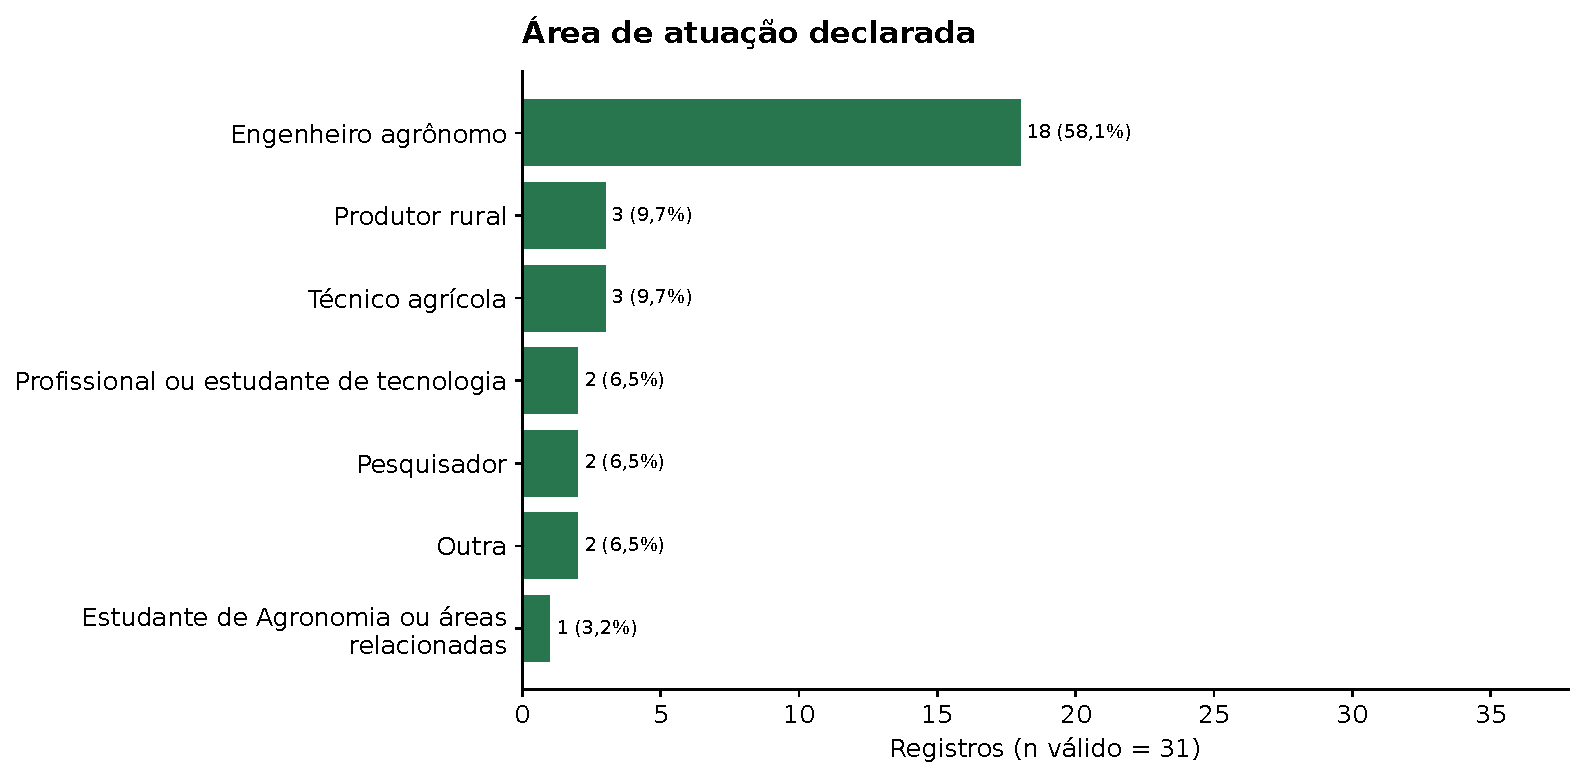
\includegraphics[width=0.82\textwidth]{avaliacao_usuarios/figuras/perfil_profissional.pdf}
\caption{Área de atuação declarada nas \UsuariosN{} submissões, conforme as categorias do instrumento.}
\label{fig:usuarios-perfil}
\fonteTCC{dados da pesquisa (2026).}
\end{figure*}

\subsubsection{Execução e experiência de uso}

A busca geográfica foi declarada concluída sem ajuda nos 32 registros. Já a demarcação apresentou a menor frequência de conclusão sem ajuda: 19/32 (59,4\%). Houve ainda cinco conclusões com auxílio, duas tentativas sem sucesso e seis respostas de não tentativa. Entre os 26 registros que indicaram tentativa, 24 informaram conclusão (92,3\%). Os dois percentuais descrevem aspectos diferentes: concluir entre quem tentou não é o mesmo que concluir sem ajuda no conjunto das respostas.

Entre as atividades tentadas, a consulta conjunta de séries e possíveis anomalias apresentou a menor proporção de conclusão: 24/29 (82,8\%), com cinco tentativas sem sucesso. Salvar uma área reuniu quatro falhas e 25/29 conclusões (86,2\%). A análise espectral teve 29/30 conclusões (96,7\%), a exploração do mapa 26/29 (89,7\%) e a consulta por cursor 25/27 (92,6\%).

Clima e exportação tiveram conclusão declarada em todas as tentativas, respectivamente 29/29 e 30/30. Porém, sete usos do clima e seis da exportação ocorreram com ajuda. Portanto, concluir a tarefa não significa necessariamente realizá-la de forma autônoma.

\begin{figure*}[htbp]
\centering
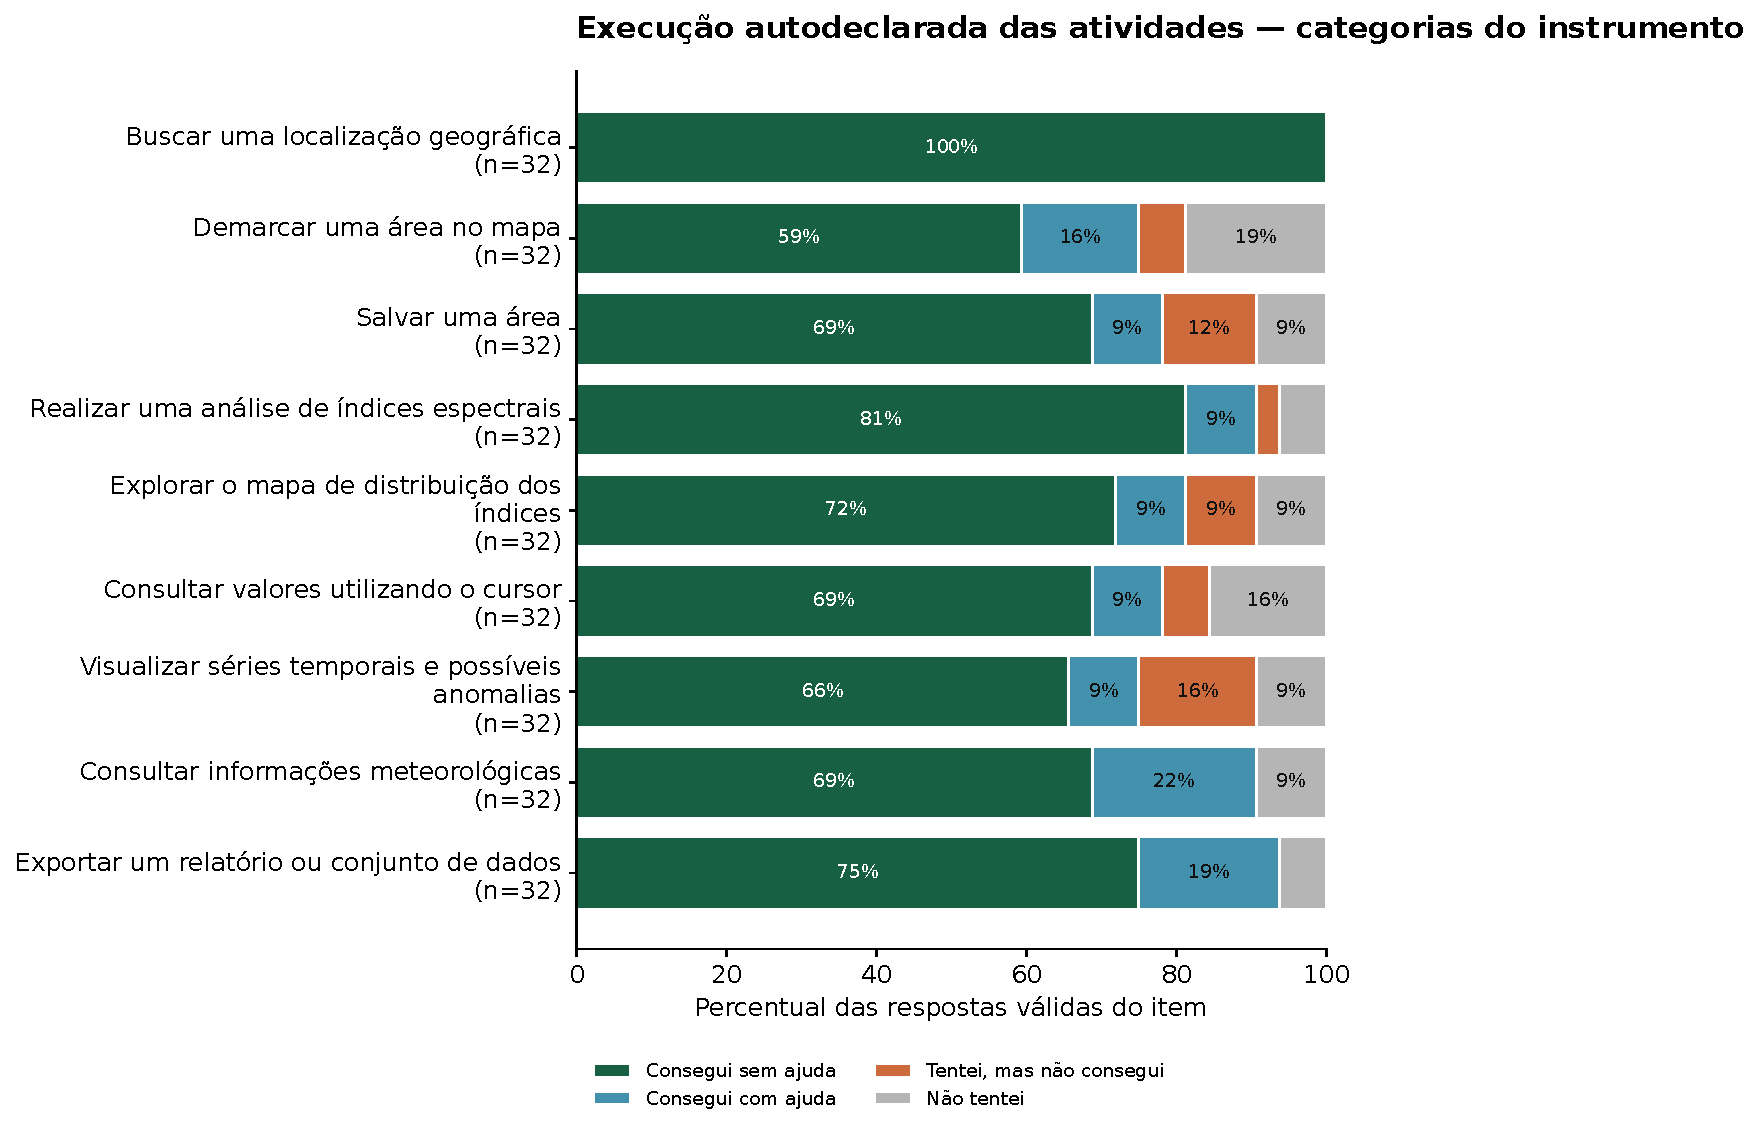
\includegraphics[width=0.98\textwidth,height=0.63\textheight,keepaspectratio]{avaliacao_usuarios/figuras/tarefas.pdf}
\caption{Execução autodeclarada das atividades, incluindo não tentativa, com base em \UsuariosN{} respostas por item.}
\label{fig:usuarios-tarefas}
\fonteTCC{dados da pesquisa (2026).}
\notaTCC{séries/anomalias e exportações mantêm o agrupamento do questionário.}
\end{figure*}

Os nove itens de experiência tiveram mediana 4, mas essa medida central não mostra todas as diferenças entre as respostas (\cref{fig:usuarios-usabilidade}). A facilidade de compreensão reuniu \UsCompreensaoPos{}/\UsCompreensaoN{} concordâncias nas categorias 4--5 (\UsCompreensaoPct\%), com uma impossibilidade de avaliação. A intuitividade teve \UsIntuitividadePos{}/\UsIntuitividadeN{} (\UsIntuitividadePct\%) e duas impossibilidades.

Quanto ao tempo de resposta, houve 22/32 concordâncias (68,8\%), oito respostas neutras e duas discordâncias. O item descreve satisfação, não uma medição do tempo de execução. A apresentação visual recebeu 23/32 concordâncias, cinco respostas neutras e quatro discordâncias. Essas diferenças permanecem relevantes mesmo quando a mediana é favorável.

\begin{figure*}[htbp]
\centering
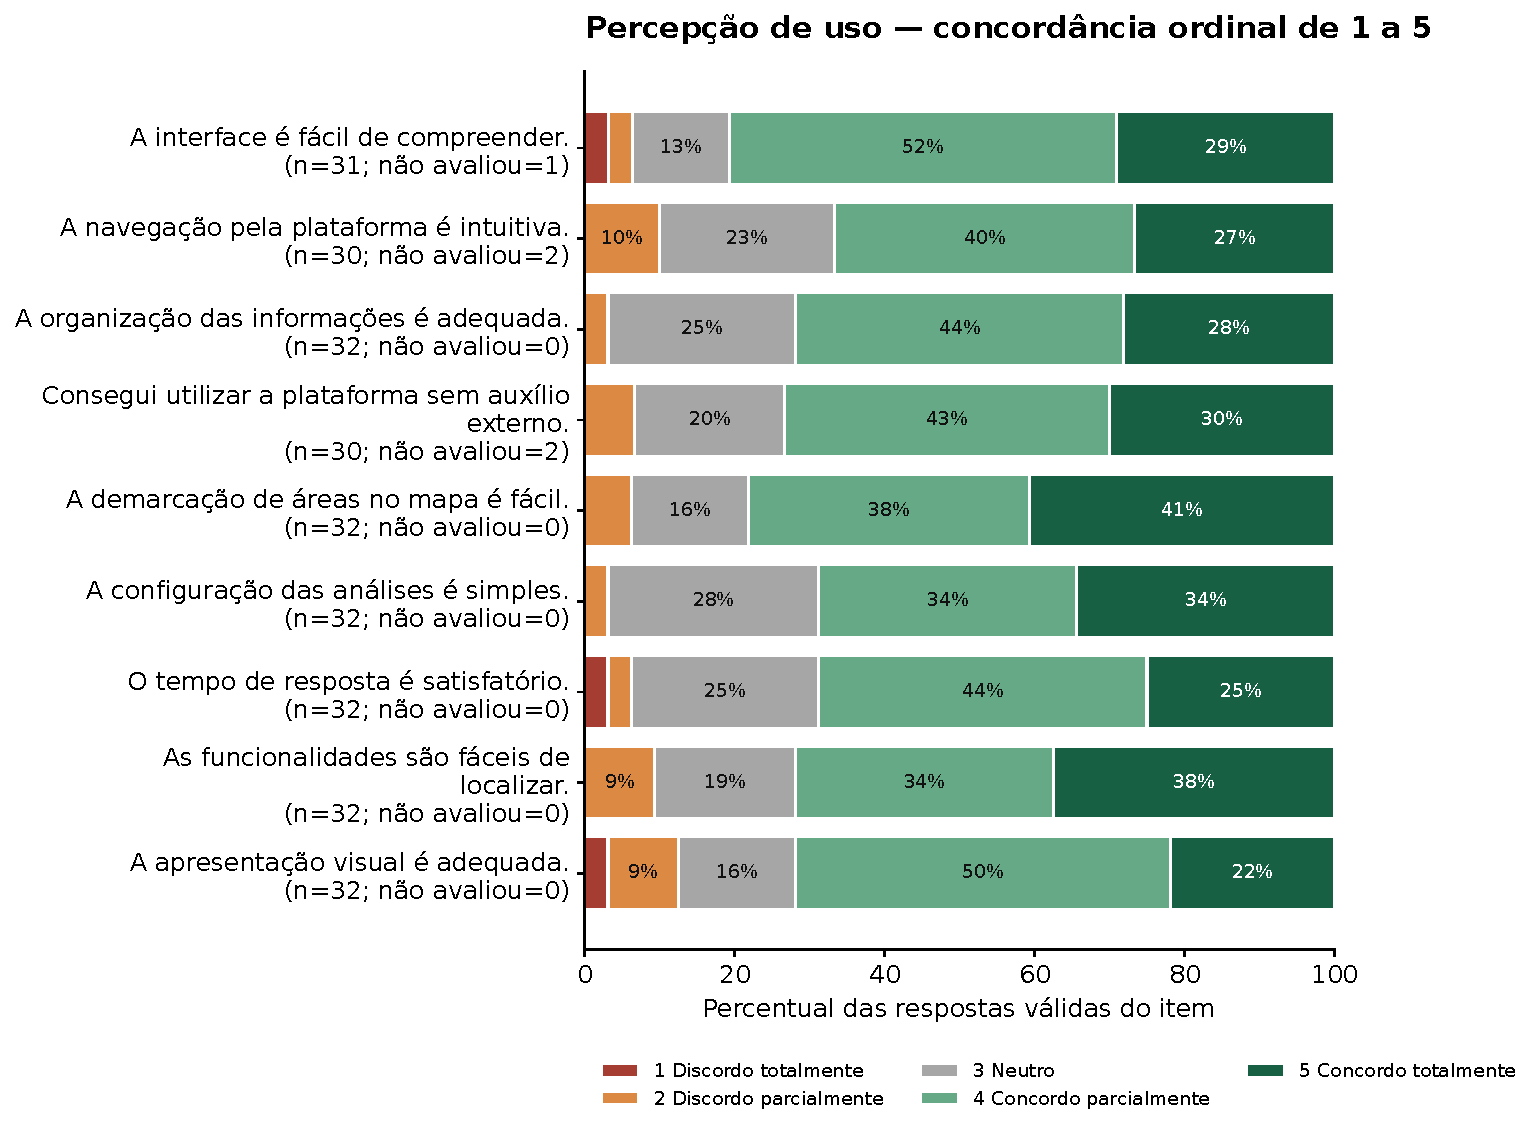
\includegraphics[width=0.98\textwidth,height=0.66\textheight,keepaspectratio]{avaliacao_usuarios/figuras/usabilidade.pdf}
\caption{Concordância sobre a experiência de uso.}
\label{fig:usuarios-usabilidade}
\fonteTCC{dados da pesquisa (2026).}
\notaTCC{cada barra apresenta as cinco categorias ordinais; o n válido exclui a impossibilidade de avaliação, informada separadamente.}
\end{figure*}

\subsubsection{Utilidade, aplicabilidade e avaliação geral}

A \cref{tab:usuarios-utilidade} apresenta os onze recursos. A consulta por pixel recebeu a maior proporção de avaliações útil/muito útil entre respostas válidas, 21/24 (87,5\%), mas oito registros não conseguiram avaliá-la. A mesma quantidade não avaliou o gerenciamento de áreas. Por isso, uma proporção alta entre avaliadores não demonstra alcance semelhante em todo o conjunto. Os mapas com gradientes tiveram mediana 5 e 25/31 avaliações 4--5; a análise espectral recebeu cinco avaliações 1--2 entre 31 válidas. Os gráficos temporais receberam 21/30 avaliações 4--5 (70,0\%).

\begin{table*}[htbp]
\centering\small
\caption{Utilidade percebida.}
\label{tab:usuarios-utilidade}
\begin{tabular}{p{0.37\textwidth}cccp{0.18\textwidth}cc}
\hline
Recurso & n & Med. & Q1--Q3 & 4--5 & 1--2 & NC\\ \hline
Busca por localização geográfica & 32 & 4 & 4,0--5,0 & 26/32 (81,2\%) & 3 & 0\\
Demarcação de áreas agrícolas & 32 & 4 & 3,0--5,0 & 22/32 (68,8\%) & 2 & 0\\
Salvamento e gerenciamento de áreas & 24 & 4 & 4,0--4,0 & 19/24 (79,2\%) & 1 & 8\\
Análise de índices espectrais & 31 & 4 & 3,0--5,0 & 21/31 (67,7\%) & 5 & 1\\
Mapas temáticos com gradientes de cores & 31 & 5 & 4,0--5,0 & 25/31 (80,6\%) & 1 & 1\\
Consulta interativa de valores por pixel & 24 & 5 & 4,0--5,0 & 21/24 (87,5\%) & 0 & 8\\
Gráficos de evolução temporal & 30 & 4 & 3,0--5,0 & 21/30 (70,0\%) & 4 & 2\\
Detecção de anomalias & 30 & 4 & 4,0--4,8 & 25/30 (83,3\%) & 1 & 2\\
Informações de temperatura e precipitação & 30 & 5 & 4,0--5,0 & 24/30 (80,0\%) & 0 & 2\\
Geração de relatórios PDF & 28 & 4 & 4,0--5,0 & 23/28 (82,1\%) & 1 & 4\\
Exportação em Excel e CSV & 27 & 4 & 4,0--4,0 & 21/27 (77,8\%) & 1 & 5\\
\hline
\end{tabular}
\fonteTCC{dados da pesquisa (2026).}
\notaTCC{Med.: mediana; Q1--Q3: quartis; 4--5: útil/muito útil; 1--2: nada/pouco útil; NC: não conseguiu avaliar. Percentuais usam o n válido do item.}
\end{table*}


Nas afirmações de aplicabilidade, 26/32 concordaram que o clima complementa a análise (81,2\%), enquanto seis entre 31 discordaram de que os gráficos facilitam o acompanhamento temporal (19,4\%). A intenção de uso profissional ou acadêmico reuniu \UsIntencaoPos{}/\UsIntencaoN{} concordâncias (\UsIntencaoPct\%), cinco respostas neutras e duas discordâncias, além de uma impossibilidade de avaliação. A recomendação teve 24/32 concordâncias (75,0\%), quatro neutras e quatro discordâncias. Esses resultados indicam percepção de aplicação e intenção, não uso continuado ou benefício agronômico demonstrado.

A nota geral teve média \UsuariosMedia{}, mediana \UsuariosMediana{}, moda \UsuariosModa{} e desvio padrão amostral \UsuariosDP{}, com \UsuariosN{} valores válidos, mínimo \UsuariosMinimo{}, máximo \UsuariosMaximo{} e quartis \UsuariosQum{} e \UsuariosQtres{}. A distribuição completa está no material complementar. Nos cruzamentos exploratórios, agrônomos tiveram mediana 4 para utilidade dos índices (n=17), contra 4,5 nas demais áreas agrupadas (n=14). A mediana da nota geral foi 8 no grupo com uso prévio frequente/ocasional (n=18) e 7,5 no grupo com poucas vezes/nunca (n=14). Os cruzamentos são descritivos, sem atribuição de efeito à profissão ou à experiência.

\subsubsection{Relatos e síntese}

Os cinco campos abertos reuniram 142 células preenchidas em 31 das 32 submissões. Os textos foram organizados em treze categorias, podendo uma mesma resposta contribuir para mais de um tema. O apoio à atividade de campo e à comunicação técnica apareceu em 30 registros, a reutilização/interoperabilidade em 19 e a relação temporal/meteorológica em 18. Esses totais incluem propostas de aplicação e de melhoria, não apenas elogios. As frequências por submissão usam o conjunto de 32 respostas; campos vazios não receberam temas.

Entre as dificuldades, treze registros mencionaram navegação, desenho ou orientação; oito, transparência dos alertas; cinco, qualidade/proveniência dos dados; e três, latência/conectividade. Dois declararam ausência de barreira relevante. A \cref{tab:usuarios-temas} relaciona categorias, trechos e implicações para o desenvolvimento.

\begin{table*}[htbp]
\centering\small
\caption{Categorias temáticas selecionadas.}
\label{tab:usuarios-temas}
\begin{tabular}{p{0.20\textwidth}cp{0.30\textwidth}p{0.34\textwidth}}
\hline
Categoria & n & Trecho literal sem identificação & Implicação\\ \hline
Representação visual e variabilidade espacial & 16 & ``Ver o mapa espacial e o gráfico temporal na mesma tela'' & Manter integração visual e comunicar limites dos índices e das cores.\\
Navegação, desenho e orientação & 17 & ``Não consegui desenhar a área sozinho'' & Priorizar orientação inicial e revisão das tarefas de demarcação e exportação.\\
Transparência e parametrização dos alertas & 13 & ``Falta clareza sobre a regra estatística'' & Explicar janela e limiar; não transformar sinalização em diagnóstico.\\
Qualidade e proveniência dos dados & 11 & ``Informar a fonte e a resolução dos dados meteorológicos'' & Expor metadados; esclarecer que NASA POWER não é estação local.\\
Latência e conectividade percebidas & 3 & ``Lentidão no carregamento de camadas raster'' & Medir latência e transferência antes de atribuir causas ou ganhos.\\
Uso móvel e acesso offline & 3 & ``Desenvolver versão otimizada para celular'' & Testar dispositivos físicos; estudar offline sem confundir com função atual.\\
\hline
\end{tabular}
\fonteTCC{dados da pesquisa (2026).}
\notaTCC{n conta registros que mencionam o tema em qualquer uma das cinco perguntas; categorias não exclusivas. Frequências completas, definições e exemplos estão no material complementar.}
\end{table*}


Alguns relatos atribuem aos mapas identificação de compactação, fertilidade ou produtividade, mencionam comparação lado a lado e alertas vermelhos/amarelos, ou pressupõem uma estação meteorológica. Esses enunciados expressam percepções e expectativas, não causas demonstradas ou recursos disponíveis. A NASA POWER fornece dados em grade, não uma estação local. A combinação de interesse declarado e interpretações imprecisas evidencia a importância de comunicar o significado dos produtos.
